% Drawing 154/08-25 -- folder 154, batch 08, archive page 156 (PDF page 157).
% Transcription: au-dessous, un croquis au crayon : deux droites $D$, $D'$ et une troisième $\Delta_s$ qui se coupent ; les orientations $\alpha$ (le long de la droite), $\beta$ (transverse) et $\omega$ (rotation), et les marques $\sigma_D$, $\sigma_{D'}$ aux extrémités d'une flèche transverse
% Kind: crossing lines with orientations alpha, beta, omega. Method 2 (schematic redraw from the facsimile). Status: partial.
% Notes: Three pencil lines: a long one rising to the right (with a thicker stretch, an arrowhead alpha beside it), a second crossing it at a marked point and running off to the upper right corner where Delta_s is written on the page (outside the crop, not drawn), a third steep one at the left. A thick transverse arrow through the crossing from the lower right, where sigma_D is written beside a marked point, to the upper left, where sigma_D' is written; a shorter arrow beside it marked beta; a curved arrow omega at the crossing and one at the lower end. Which of the pencil lines is D and which D' is not written in the sketch; the letters are left out. Labels as the transcription reads them. Redrawn 2026-11-12 (issue 128): to check again.
% Coordinates: 1 unit = 1 mm = 1/100 of the crop width (bbox in page fractions: [0.1, 0.205, 0.235, 0.3]).
% Redrawn by Claude (claude-fable-5-2), issue #128, 2026-11-12; not checked by a human; not compiled (no TeX in the session).
% Rights: reproduces part of the work -- behind RENDER_TRANSCRIPTS, never published by itself.
\documentclass[tikz,border=3pt]{standalone}
\usepackage{amsmath,amssymb}
\usetikzlibrary{patterns,arrows.meta}
\tikzset{pencil/.style={black!45}, struck/.style={black!35}, mpt/.style={circle,draw,inner sep=1.3pt}, pt/.style={circle,fill,inner sep=0.9pt}, opt/.style={circle,draw,fill=white,inner sep=1.1pt}}
\begin{document}
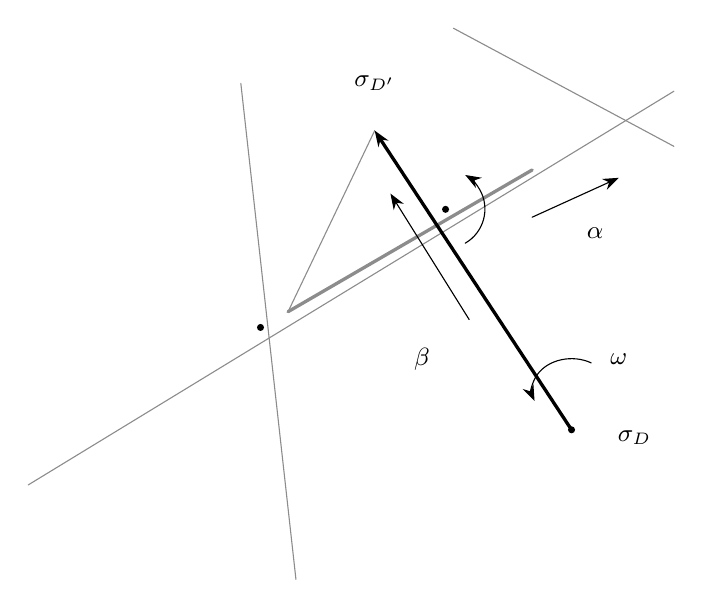
\begin{tikzpicture}[x=1mm,y=1mm,line cap=round,line join=round,font=\scriptsize]
\draw[pencil] (16,-86) -- (98,-36);
\draw[pencil,very thick] (49,-64) -- (80,-46);
\draw[pencil] (70,-28) -- (98,-43);
\draw[pencil] (43,-35) -- (50,-98);
\draw[pencil] (49,-64) -- (60,-41);
\draw[very thick,-{Stealth[length=2mm]}] (85,-79) -- (60,-41);
\draw[-{Stealth[length=2mm]}] (72,-65) -- (62,-49);
\draw[-{Stealth[length=2mm]}] (80,-52) -- (91,-47);
\node[pt] at (69,-51) {};
\node[pt] at (85,-79) {};
\node[pt] at (45.5,-66) {};
\draw[-{Stealth[length=2mm]}] (71.5,-55.3) arc[start angle=300, end angle=420, x radius=5, y radius=5];
\draw[-{Stealth[length=2mm]}] (87.5,-70.5) arc[start angle=60, end angle=200, x radius=5, y radius=4];
\node[inner sep=1pt] at (60,-35) {\small $\sigma_{D'}$};
\node[inner sep=1pt] at (93,-80) {\small $\sigma_D$};
\node[inner sep=1pt] at (66,-70) {\small $\beta$};
\node[inner sep=1pt] at (88,-54) {\small $\alpha$};
\node[inner sep=1pt] at (91,-70) {\small $\omega$};
\end{tikzpicture}
\end{document}
